\documentclass[aspectratio=169]{beamer}
% Shared preamble for ml/ slide decks.
% Each lecture .tex starts with:
%   \documentclass[aspectratio=169]{beamer}
%   \input{../preamble}
% Compile from inside the chapter folder so \input{../preamble} resolves.

\usetheme{default}
\usecolortheme{dove}

\setbeamertemplate{navigation symbols}{}
\setbeamertemplate{footline}{%
  \hfill{\large\insertframenumber\,/\,\inserttotalframenumber}\hspace{0.8em}\vspace{0.5em}%
}

% Project palette (existing, kept for backwards compatibility with deferred/*)
\definecolor{popblue}{RGB}{52, 101, 164}
\definecolor{sampred}{RGB}{204, 0, 0}
\definecolor{paramgreen}{RGB}{0, 140, 70}
\definecolor{warnred}{RGB}{180, 40, 40}
\definecolor{orange1}{RGB}{220, 120, 0}
\definecolor{violet1}{RGB}{120, 50, 160}
\definecolor{lightbg}{RGB}{245, 245, 250}

% Armenian flag palette (use these for any 3-color highlight; per CLAUDE.md).
% "Nice versions": slightly de-saturated from the official spec for slide use,
% so they don't burn out under projector colors. Originals kept as *_pure.
\definecolor{armred}{RGB}{200, 30, 40}      % nice red (official #D90012 muted)
\definecolor{armblue}{RGB}{30, 70, 160}     % nice blue (official #0033A0 muted)
\definecolor{armorange}{RGB}{230, 160, 30}  % nice orange (official #F2A800 muted)
\definecolor{armred_pure}{HTML}{D90012}     % official Armenian flag red
\definecolor{armblue_pure}{HTML}{0033A0}    % official Armenian flag blue
\definecolor{armorange_pure}{HTML}{F2A800}  % official Armenian flag orange

\setbeamercolor{frametitle}{fg=popblue}
\setbeamercolor{title}{fg=popblue}

\usepackage{pgfplots}
\usepackage{tikz}
\usetikzlibrary{shapes, arrows.meta, positioning, calc, decorations.pathreplacing, patterns, matrix}
\pgfplotsset{compat=1.18}
\usepackage{amsmath, amssymb, amsfonts}
\usepackage{bm}
\usepackage{dsfont}
\usepackage{array}
\usepackage{pifont}
\usepackage{colortbl}
\usepackage{fontenc}

% Callout boxes. Purely additive - existing decks are unaffected.
% Usage: \begin{tcolorbox}[colback=armblue!8, colframe=armblue, boxrule=0.6pt, arc=2pt,
%                          title=\textbf{Key idea}] ... \end{tcolorbox}
% Palette convention (ml/SLIDE_STYLE.md): armblue=key idea, armred=trap/warning,
% paramgreen=takeaway or "Next", armorange=watch-out.
\usepackage[most]{tcolorbox}

% Cleaner table rules (\toprule, \midrule, \bottomrule). Also purely additive.
\usepackage{booktabs}

% \cancel{...} for struck-through terms in derivations (added 2026-08-11 for the
% importance-sampling frame in ch11_rl, where the dynamics cancel). Purely additive.
\usepackage{cancel}

% Minimal ML notation macros (subset of slds-lmu latex-math/basic-ml.tex).
% Kept here so we don't have to inline-expand every \thetav, \xv, etc.
% when porting upstream slides.
\newcommand{\R}{\mathds{R}}
\newcommand{\N}{\mathds{N}}
\newcommand{\E}{\mathds{E}}
\newcommand{\Xspace}{\mathcal{X}}
\newcommand{\Yspace}{\mathcal{Y}}
\newcommand{\Hspace}{\mathcal{H}}
\newcommand{\D}{\mathcal{D}}
\newcommand{\Dtrain}{\mathcal{D}_{\text{train}}}
\newcommand{\Dtest}{\mathcal{D}_{\text{test}}}
\newcommand{\xv}{\mathbf{x}}
\newcommand{\yv}{\mathbf{y}}
\newcommand{\Xmat}{\mathbf{X}}
\newcommand{\id}{\mathbf{I}}
\newcommand{\thetav}{\bm{\theta}}
\newcommand{\thetah}{\hat{\bm{\theta}}}
\newcommand{\lamv}{\bm{\lambda}}
\newcommand{\fx}{f(\xv)}
\newcommand{\fxt}{f(\xv \,|\, \bm{\theta})}
\newcommand{\fxi}{f\!\left(\xv^{(i)}\right)}
\newcommand{\fh}{\hat{f}}
\newcommand{\fxh}{\hat{f}(\xv)}
\newcommand{\yh}{\hat{y}}
\newcommand{\yih}{\hat{y}^{(i)}}
% \xi clashes with the Greek letter \xi; write \xv^{(i)} inline instead.
\newcommand{\yi}[1][i]{y^{(#1)}}
\newcommand{\xyi}[1][i]{\left(\xv^{(#1)},\, y^{(#1)}\right)}
\newcommand{\thx}{\bm{\theta}^\top \xv}
\newcommand{\sumin}{\sum_{i=1}^{n}}
\newcommand{\sumjp}{\sum_{j=1}^{p}}
\newcommand{\Lxy}{L\!\left(y, \fx\right)}
\newcommand{\Lxyi}{L\!\left(\yi, \fxi\right)}
\newcommand{\risk}{\mathcal{R}}
\newcommand{\riske}{\mathcal{R}_{\text{emp}}}
\newcommand{\risket}{\mathcal{R}_{\text{emp}}(\bm{\theta})}
\newcommand{\riskt}{\mathcal{R}(\bm{\theta})}
\newcommand{\riskr}{\mathcal{R}_{\text{reg}}}
\newcommand{\argmin}{\mathop{\mathrm{arg\,min}}}
\newcommand{\argmax}{\mathop{\mathrm{arg\,max}}}
\newcommand{\eps}{\varepsilon}


\graphicspath{{fig/}{../00_shared/fig/}}

% callout boxes, matching the chapter's fcolorbox house pattern (LLM-1 to LLM-8)
\newcommand{\keybox}[1]{\fcolorbox{armblue}{armblue!8}{\parbox{0.97\linewidth}{\small #1}}}
\newcommand{\trapbox}[1]{\fcolorbox{armred}{armred!8}{\parbox{0.97\linewidth}{\small #1}}}
\newcommand{\takebox}[1]{\fcolorbox{paramgreen}{paramgreen!8}{\parbox{0.97\linewidth}{\small #1}}}
\newcommand{\watchbox}[1]{\fcolorbox{armorange}{armorange!12}{\parbox{0.97\linewidth}{\small #1}}}

\newcommand{\sectiontransition}[2]{%
  \begin{frame}[plain]
    \vfill
    \begin{center}
      {\Huge\bfseries\color{popblue} #1}\\[1.1em]
      {\large #2}
    \end{center}
    \vfill
  \end{frame}}

\newcommand{\src}[1]{{\scriptsize\color{gray} #1}}

\title{Post-training}
\subtitle{From a base model to an assistant}
\author{}
\date{}

\begin{document}

\begin{frame}[plain]
  \titlepage
  \begin{center}\scriptsize\color{gray}
    LLM chapter, session 9. Toy numbers unless a slide says otherwise.
  \end{center}
\end{frame}

% ============================================================ WHERE WE ARE (py_src/llm_roadmap.py)
\begin{frame}{Where we are: one forward pass}
  \begin{center}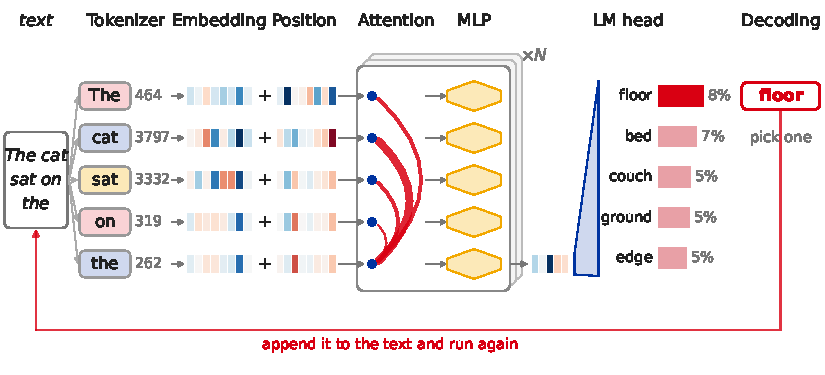
\includegraphics[width=\linewidth]{roadmap_post_training_pass.pdf}\end{center}
  \vskip -2pt
  {\small Same pass, same kind of weights. Today changes only \emph{which} continuation it prefers.}
\end{frame}

\begin{frame}{Where we are: the life of a model}
  \begin{center}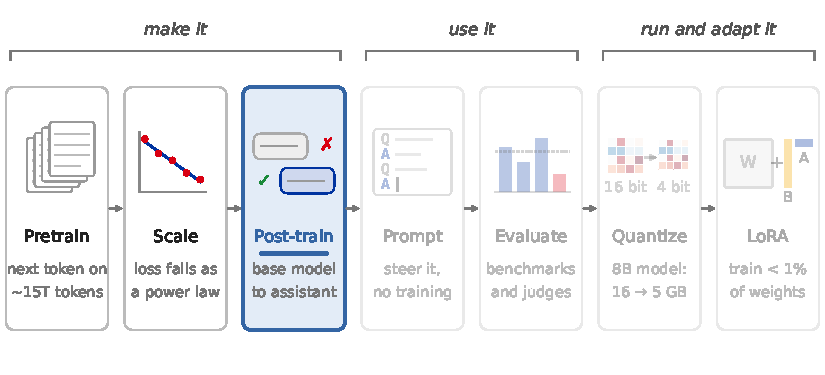
\includegraphics[width=\linewidth]{roadmap_post_training_life.pdf}\end{center}
  \vskip -2pt
  {\small Today: the third box. LLM-7 ended with a base model that continues documents.}
\end{frame}

% ============================================================ COLD OPEN (py_src/posttrain_figs.py --gpt2)
\begin{frame}{Ask a base model}
  \vskip 8pt
  GPT-2 small is a base model: pretrained (LLM-7), nothing else. Give it one line:

  \vskip 12pt
  \begin{center}
    \fbox{\parbox{0.6\linewidth}{\centering\ttfamily How do I reset my password?}}
  \end{center}

  \vskip 14pt
  \trapbox{\textbf{Predict first:} what does it write next? (Greedy, the next 50 tokens.)}
\end{frame}

\begin{frame}{It writes an FAQ page}
  \begin{center}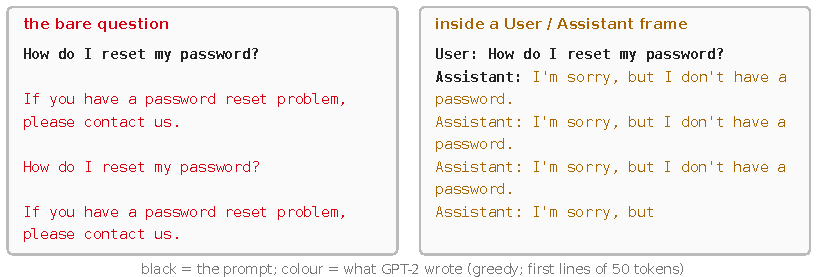
\includegraphics[width=0.86\linewidth]{post_cold_open.pdf}\end{center}
  \vskip -4pt
  {\small Left: it writes the page around the question - a canned reply, then the same question
  again, in a loop. Right: given a User / Assistant frame it does play the assistant, but
  unhelpfully, and it never stops: it writes the next ``Assistant:'' turn itself.}

  \vskip 4pt
  \keybox{The base model is not missing knowledge here; it is missing a \emph{habit}. Its most
  likely continuation of a question is more web page. Post-training changes which continuation
  is most likely.}
\end{frame}

\begin{frame}{Outline}
  \tableofcontents
\end{frame}

\begin{frame}{Three ways to change a habit}
  \begin{center}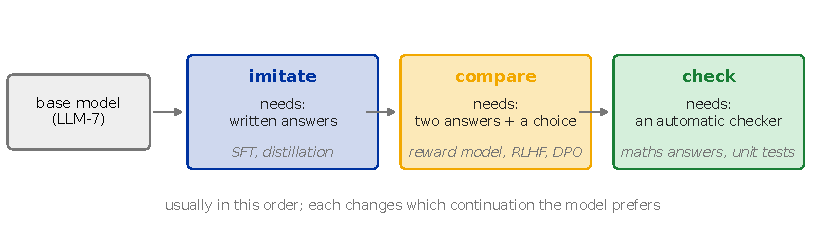
\includegraphics[width=\linewidth]{post_three_verbs.pdf}\end{center}
  \vskip -2pt
  {\small All three keep the architecture and the next-token machinery. They differ in what the
  training signal is made of - and so in what they cost and what can go wrong.}
\end{frame}

% ============================================================ 1. IMITATE
\section{Imitate}
\sectiontransition{Imitate}{Show it thousands of good conversations.}

\begin{frame}{Supervised fine-tuning (SFT)}
  \vskip 4pt
  \begin{itemize}
    \item Hire people (``labelers'') to write conversations: a prompt, then the answer a helpful
      assistant should give, following written guidelines.
    \item Train on them with \textbf{LLM-7's loss}: the next token, $-\ln p$. Only the
      \emph{assistant's} tokens are scored; the user's turn is context.
    \item Tens of thousands of conversations instead of trillions of tokens: hours of training,
      not months.
  \end{itemize}

  \vskip 8pt
  \keybox{What you talk to is, in Karpathy's words, ``a simulation of a human labeler'': the
  model learned what a labeler following those guidelines would most likely write.}
  \src{Karpathy, ``Deep Dive into LLMs like ChatGPT'' (2025).}
\end{frame}

\begin{frame}{The chat template}
  \begin{center}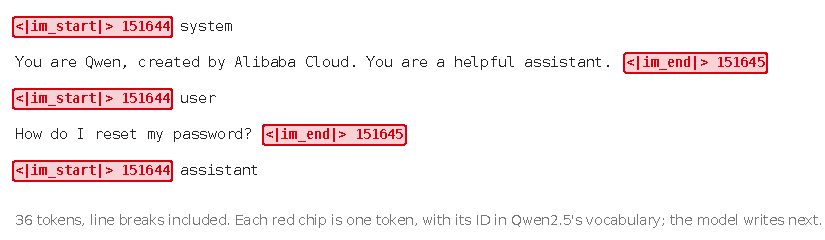
\includegraphics[width=\linewidth]{post_chatml.pdf}\end{center}
  \vskip -4pt
  {\small A conversation still has to be \emph{one} token stream: Qwen2.5's format (ChatML),
  tokenized by its own tokenizer. Special tokens (LLM-1) mark who speaks; the system turn is the
  default Qwen inserts when you give none. In SFT only the assistant's turns are scored.}

  \vskip 4pt
  \takebox{The model learns to end its turn with \texttt{<|im\_end|>}, so the app knows when to
  stop (LLM-6). Without its template, a chat model drifts back towards continuing documents.}
\end{frame}

\begin{frame}{How much data?}
  \vskip 2pt
  \begin{itemize}
    \item \textbf{Breadth} - FLAN (Wei et al., 2021): 62 existing datasets rewritten as
      instructions. Zero-shot, the 137B model beat zero-shot GPT-3 (175B) on 20 of 25 datasets.
      But in models of 8B and below the same tuning \emph{hurt}: they had no room to spare.
    \item \textbf{Quality} - LIMA (Zhou et al., 2023): LLaMa 65B fine-tuned on only
      \textbf{1,000} carefully chosen examples. People judged its answers equivalent to or better
      than GPT-4's in 43\% of cases.
  \end{itemize}

  \vskip 8pt
  \keybox{LIMA's reading: almost all the knowledge comes from pretraining. Post-training mostly
  teaches the format and the style of a good answer - which is why a little of it goes a long
  way.}
\end{frame}

\begin{frame}{Imitating a bigger model}
  \vskip 6pt
  \textbf{Distillation} is SFT where the ``labeler'' is another model:
  \begin{itemize}
    \item a large, strong model (the teacher) writes answers to many prompts;
    \item a small model (the student) is fine-tuned on them with the same loss.
  \end{itemize}

  \vskip 6pt
  DeepSeek-R1 (2025) was distilled into smaller Qwen and Llama models with about
  \textbf{800,000} of its own samples (600k reasoning, 200k other).

  \vskip 10pt
  \watchbox{A student imitates the teacher's habits, including its mistakes. It can approach the
  teacher; imitation alone does not take it beyond - unless a checker supplies a new signal (the
  last section).}
\end{frame}

% ============================================================ 2. COMPARE
\section{Compare}
\sectiontransition{Compare}{Judging is easier than writing.}

\begin{frame}{Why compare}
  \vskip 6pt
  \begin{itemize}
    \item Writing the perfect answer to every prompt is slow and hard. Saying which of two answers
      is better is fast, and people agree on it more often.
    \item So: let the model write two answers, A and B, and have a person pick one. Thousands of
      such \textbf{preference pairs}.
    \item Then train a \textbf{reward model}: a copy of the network with a single number on top,
      $r(\text{prompt}, \text{answer})$, high for answers people prefer - with the loss on the next
      page.
  \end{itemize}

  \vskip 10pt
  \keybox{A reward model turns ``A is better than B'' into a score that can grade answers no person
  has seen.}
\end{frame}

\begin{frame}{Bradley-Terry, by hand}
  \begin{columns}[c]
    \column{0.58\textwidth}
      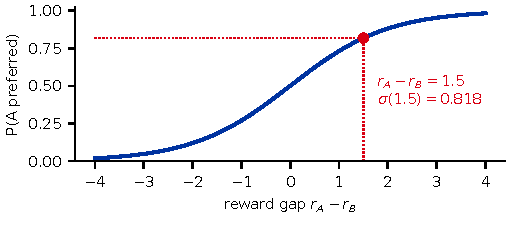
\includegraphics[width=\linewidth]{post_bradley_terry.pdf}
    \column{0.40\textwidth}
      {\small Toy numbers. The reward model scores two answers: $r_A = 2.0$, $r_B = 0.5$.
      \vskip 4pt
      $P(A \text{ preferred}) = \sigma(r_A - r_B) = \sigma(1.5) = \mathbf{0.818}$
      \vskip 4pt
      ($\sigma$: the sigmoid. Only the gap matters - as with logits in LLM-5.)}
  \end{columns}

  \vskip 8pt
  {\small \textbf{Training it:} if people chose A, the loss is $-\ln 0.818 = 0.20$; if they chose
  B, it is $-\ln(1 - 0.818) = -\ln 0.182 = 1.70$, and the gradient pushes $r_B$ up and $r_A$
  down.}
  \vskip 4pt
  \keybox{The same $-\ln p$ as everywhere in this chapter, on one comparison at a time.}
\end{frame}

\begin{frame}{RLHF in one picture}
  \begin{center}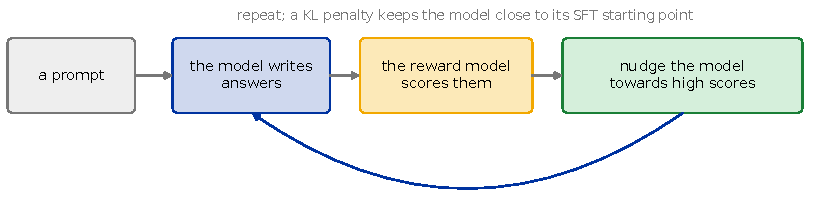
\includegraphics[width=\linewidth]{post_rlhf.pdf}\end{center}
  \vskip -2pt
  \begin{itemize}
    \small
    \item RLHF, reinforcement learning from human feedback: the reward model stands in for the
      people, so the loop can run millions of times.
    \item The nudge: raise the probability of the tokens in high-scoring answers, lower it in
      low-scoring ones. The algorithm (PPO) is the reinforcement-learning chapter's.
    \item The KL penalty: KL divergence is 0 when two probability distributions are identical and
      grows as they differ. Charging for it keeps the model near the SFT model: a leash.
  \end{itemize}
\end{frame}

\begin{frame}{It works: 1.3B beats 175B}
  \vskip 10pt
  InstructGPT (Ouyang et al., 2022): GPT-3 after SFT and RLHF.

  \vskip 10pt
  \begin{center}
    \fcolorbox{paramgreen}{paramgreen!8}{\parbox{0.8\linewidth}{\centering
    People preferred the answers of the \textbf{1.3B} InstructGPT to those of the \textbf{175B}
    GPT-3 - a model over 100$\times$ larger.}}
  \end{center}

  \vskip 10pt
  {\small At equal size the gap is wider: head to head, the 175B InstructGPT beat the 175B GPT-3
  85\% of the time.}

  \vskip 6pt
  \keybox{Same pretraining data and recipe at a smaller size, preferred anyway. For the people
  asking, the habit mattered more than the size. (ChatGPT grew out of this model family.)}
\end{frame}

\begin{frame}{Reward hacking}
  \begin{columns}[c]
    \column{0.58\textwidth}
      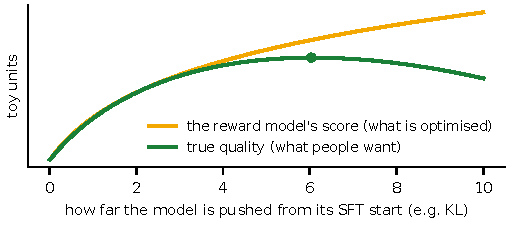
\includegraphics[width=\linewidth]{post_goodhart.pdf}
    \column{0.40\textwidth}
      {\small Toy curves, the shape Gao et al. (2022) measured: push a model hard enough towards
      a reward model's score and the score keeps rising while real quality falls.}
  \end{columns}

  \vskip 8pt
  \trapbox{The reward model is a proxy, trained on a few thousand comparisons. Optimise it too
  hard and the model finds what the proxy over-rewards (longer answers, confident tone, flattery)
  instead of what people wanted. Goodhart's law: when a measure becomes a target, it stops being
  a good measure. The KL leash limits how far the model can be pushed - ideally stopping it near
  the peak, not past it.}
\end{frame}

\begin{frame}{DPO: skip the reward model}
  \vskip 6pt
  Rafailov et al. (2023), Direct Preference Optimization:
  \begin{itemize}
    \item Keep the preference pairs; drop the separate reward model and the RL loop.
    \item The model's own probabilities play the reward's role. For each answer, take
      $\Delta = \ln p_{\text{model}}(\text{answer}) - \ln p_{\text{ref}}(\text{answer})$: how much
      more likely the model makes it than a frozen copy of the SFT model does.
    \item The loss is Bradley-Terry again, with $\Delta$ in place of $r$:
      $-\ln \sigma\big(\beta\,(\Delta_{\text{chosen}} - \Delta_{\text{rejected}})\big)$, where
      $\beta$ sets how far the model may move.
  \end{itemize}

  \vskip 10pt
  \keybox{One supervised-style training run instead of three stages. Much of open-model
  preference tuning uses DPO or its variants; the derivation is the reinforcement-learning
  chapter's.}
\end{frame}

% ============================================================ 3. CHECK
\section{Check}
\sectiontransition{Check}{When an answer can be checked, the checker is the teacher.}

\begin{frame}{Verifiable rewards}
  \vskip 4pt
  \begin{itemize}
    \item Some answers can be checked by a program: a maths answer against the known result,
      code against unit tests.
    \item Then no person and no reward model are needed: the program's verdict is the reward.
    \item DeepSeek-R1-Zero (2025) used two rule-based rewards: is the answer correct, and is the
      reasoning written between \texttt{<think>} and \texttt{</think>} tags (a format reward). The
      authors avoided a neural reward model because it ``may suffer from reward hacking''.
  \end{itemize}

  \vskip 8pt
  \keybox{Reasoning models such as DeepSeek-R1 are trained this way: long chains of thought that
  end in a checkable answer (LLM-8's second axis). The details are the reinforcement-learning
  chapter's.}
\end{frame}

% ============================================================ CLOSE
\begin{frame}{Recap}
  \small
  \begin{itemize}
    \item A base model has the knowledge but the wrong habit: it continues documents.
    \item \textbf{Imitate}: SFT on written conversations (one chat template, special tokens);
      quality beats quantity (LIMA); distillation imitates a bigger model.
    \item \textbf{Compare}: preference pairs $\to$ a reward model (Bradley-Terry:
      $\sigma(r_A - r_B)$) $\to$ RLHF with a KL leash; DPO skips the reward model. A 1.3B
      InstructGPT beat a 175B GPT-3.
    \item \textbf{Reward hacking}: optimise a proxy too hard and quality falls.
    \item \textbf{Check}: when a program can verify the answer, it is the reward.
  \end{itemize}
\end{frame}

\begin{frame}{Next on the map}
  \begin{center}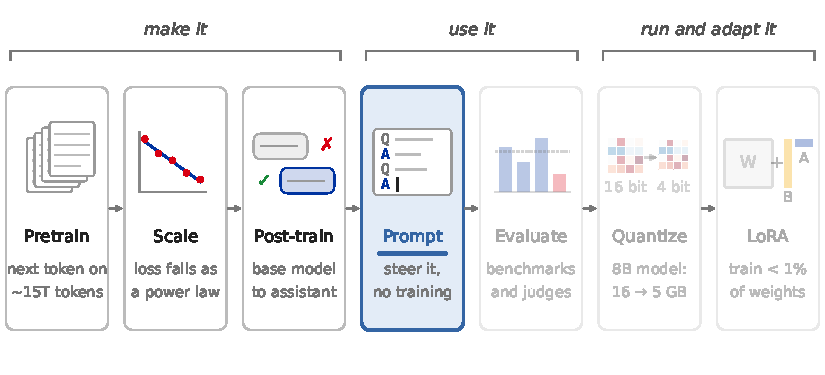
\includegraphics[width=\linewidth]{roadmap_prompting_life.pdf}\end{center}
  \vskip -2pt
  {\small Next (LLM-10): prompting - steering a trained model with nothing but the text you give
  it.}
\end{frame}

\begin{frame}{Sources \& further reading}
  \footnotesize
  \begin{itemize}
    \item Ouyang et al. (2022), ``Training language models to follow instructions with human
      feedback'' (InstructGPT).
    \item Wei et al. (2021), ``Finetuned Language Models Are Zero-Shot Learners'' (FLAN); Zhou et
      al. (2023), ``LIMA: Less Is More for Alignment''.
    \item Gao, Schulman \& Hilton (2022), ``Scaling Laws for Reward Model Overoptimization''.
    \item Rafailov et al. (2023), ``Direct Preference Optimization''.
    \item DeepSeek-AI (2025), ``DeepSeek-R1''; Qwen2.5 model card and tokenizer configuration.
    \item Karpathy (2025), ``Deep Dive into LLMs like ChatGPT''.
  \end{itemize}
  \vskip 2pt
  \src{Figures: \texttt{py\_src/posttrain\_figs.py}. Real: GPT-2's two continuations (cached model,
  one run) and the ChatML conversation tokenized with Qwen2.5's cached tokenizer. Toy: the
  Bradley-Terry numbers and the reward-hacking curves.}
\end{frame}

\end{document}

% ============================================================================
% Provenance:
%   Deck: LLM-9 Post-training (14_llms), session 9. Built 2026-10-06 from
%   LLM9_post_training_OUTLINE.md, which follows the critique in LLM_CHAPTER_PLAN.md (LLM-9) and
%   the recommended answers in INTERVIEW_QUEUE.md (instructor: "do all queue items"): the
%   imitate / compare / check spine, the GPT-2 password cold open, Bradley-Terry by hand
%   (2.0 vs 0.5 -> 0.82), reasoning models as a teaser. Idea level for RLHF and DPO (D3).
%   Sources ported: dl4nlp 07 sections 2-4; llm_training 10 (InstructGPT), 18 (FLAN), 04 (LIMA);
%   distillation from dl4nlp 11 (the 800k samples, re-checked in the R1 paper).
%   Facts checked 2026-10-06: the outline's table (LIMA and Gao abstracts, the R1 full text,
%   Qwen2.5's tokenizer_config.json, the local FLAN and InstructGPT decks, Karpathy's transcript).
%   Not available locally: an instruction-tuned model (only Qwen2.5's tokenizer.json is cached),
%   so the cold open shows GPT-2 bare and GPT-2 in a User / Assistant frame; downloading an
%   instruct model for a side-by-side is left to the instructor.
%   STUDENT REVIEW 2026-10-06 (one Sonnet agent, rendered PNGs only; ~77k tokens, 60 s). Caught:
%   "-ln 0.18 = 1.70" does not follow from the printed 0.18 (it is 1.71); now three decimals,
%   0.818 / 0.182 -> 0.20 / 1.70, checked from the printed values. Applied: DPO's loss written out
%   with the frozen SFT reference; the RLHF nudge made concrete, KL defined, "policy" dropped; the
%   36 tokens include line breaks; no overclaim about untemplated chat models; the 85% head-to-head
%   (local InstructGPT deck); R1-Zero's correctness and format rewards; the KL leash tied to the
%   curve; a forward pointer for the reward model's loss; darker orange and larger labels.
% ============================================================================
